\graphicspath{{chapters/4.Chapter2/figures/}}

\begin{savequote}[75mm]
"even after the observation of the frequent or constant conjunction of objects, we have no reason to draw any inference concerning any object beyond those of which we have had experience;"
\qauthor{- David Hume: \textit{A Treastie of Human Nature, 1738}}
\end{savequote}

% what about negative samples 

\chapter{Transcriptomic analysis of the \textit{Paramecium bursaria} and \textit{Micractinium reisseri} endosymbiosis}

\section{Introduction}

Transcriptomics, and specifically RNAseq, is a powerful method by which the \textit{Paramecium bursaria}-\textit{Micractinium reisseri} (PbMr)
endosymbiosis can be investigated. This endosymbiosis conveys phototrophy \citep{Karakashian1963} as well as 
numerous photobiological behavioural and biochemical traits (e.g. \citep{Berk1991,Saji1974,Nakajima1989,Niess1982a,Iwatsuki1988,Summerer2009}, 
partially reviewed in \citep{Sommaruga2009}).  Photosynthesis and unidentified light-induced factors have been identified as key to the establishment
and maintenance of this endosymbiosis (and prevention of algal digestion by the host) \citep{Karakashian1963,Hosoya1995a,Kodama2007,Kodama2014c}.
Therefore, a (relatively) unbiased global metatranscriptomic profile of host and endosymbiont in both lit and dark conditions can be used to 
identify key transcripts playing a role in the establishment, maintenance, and photobiological traits of this endosymbiosis. 
%constitutively expressed photosynthetic components
%This profile will allow metabolic reconstruction of host and endosymbiont in both photosynthetically active and inactive
%states as well as offering a means to identify significantly differentially expressed transcripts between these states.


The effectiveness of this type of approach is evidenced by several studies investigating
host-chloroplast interactions \citep{Nowack2011,Jiggins2013,Xiang2015}. 
Studies of the interaction between a small number of defined organisms e.g. host-endosymbiont, host-pathogen etc.
fall between the full large scale environmental transcriptomics of microbial ecology \citep{Poretsky2005,AliagaGoltsman2014} 
and the large axenic cultures of traditional transcriptomics.  This type of study has been dubbed
as ``dual-RNAseq'' \citep{Westermann2012}, particularly in the area of host-pathogen interactions \citep{Tieryney2012}.


\textit{Paramecium bursaria} and its green algal endosymbionts are particularly well suited for investigation
using a ``dual-RNAseq'' approach.  This is due to the plethora of 
of literature on the physiology and behaviour of host and endosymbiont, both together and individually.
(e.g. \citep{Iwatsuki1988}, see \citep{Kato2009a} and \ref{chap:introduction} for more details).
On top of this, there is evidence of transcriptomic tractability in reasonably close relatives of both organisms 
(for example, \citep{Guarnieri2011,Rowe2014,Bashan2015} and \citep{Arnaiz2010,Kolisko2014}), as well as
one published analysis of host transcriptome with and without a \textit{Chlorella} endosymbiont \citep{Kodama2014}.
Unfortunately, this system is also genomically complex, with \textit{P. bursaria}'s classical ciliate nuclear
dimorphism, sexual reproduction, partially digested bacterial prey foodstock, and range of associated
bacterial and viral organisms.  There are also no available reference genomes for either \textit{Paramecium bursaria} or \textit{Micractinium reisseri}.
However, sequenced genomes for other divergent ciliates (i.e. \textit{Tetrahymena thermophila} \citep{Eisen2006} and \textit{Paramecium caudatum}
\citep{McGrath2014}) and for fairly closely related algae \textit{Chlorella variabilis} NC64A \citep{Blanc2010} and \textit{Coccomyxa subellipsoidea} C-169 \citep{Blanc2012}
(see \ref{fig:introduction} and \ref{fig:introduction}), %phylogenies in introduction
which could potentially aid transcriptome assembly.  
It should be noted that \citep{Kodama2014}, \citep{Kolisko2014} and \citep{Guarnieri2011} all recapitulated 
\textit{Paramecium bursaria}, another \textit{Paramecium} species, and \textit{Chlorella vulgaris} transcriptomes \textit{de novo} (without a reference genome).


Towards this end we conducted a bulk RNAseq sequencing of cultured PbMr using 76bp paired-end reads and the Illumina Gene Analyzer II platform.
Unfortunately, due to limitations in the maintainable culture density of the \textit{Paramecium bursaria} CCAP 1660/12 and thus the quantity of extractable
mRNA it was necessary to pool all day and night replicates into a single pair of day and night libraries. 
While this provided sufficient material for sequencing it precluded accurate inference of significant differential expression between day or night
as it masked all biological replicates \citep{Auer2010}.  We, therefore, also sequenced a set of 3 (followed later by an additional 5) dark and 3 light
biological replicates using single-cell RNAseq (sc-RNAseq) methods. 


sc-RNAseq are a relatively new set of technologies which facilitate transcriptome sequencing with starting material on the range of picograms
derived from 1 to a few cells (reviewed \citep{Macaulay2014,Liang2014,Wu2014a}).  There are a range of sc-RNAseq methodologies 
(covered in \ref{chap:methods}) e.g. Quartzseq \citep{Sasagawa2013}, Tang's method \citep{Tang2009} and SMARTSEQ \citep{Goetz2012,Picelli2014},
however we used the poly-A reverse transcription multiple displacement amplification (MDA) based method \citep{Korfhage2015}.  
This method was selected as its based method (MDA) has already been widely applied and characterised in single cell genomics (e.g. \citep{Spits2006}),
and it is relatively simple and reliable.  \textbf{Need to add more to this <>}  

%Although not exlcusive to MDA based sc-RNAseq, this method
%can improve 3' resolution of transcripts.  It was observed in preliminary bulk assemblies that both C- and N- terminal coverage 
%in transcripts was limited.  As accurate identification of secreted peptides hinges on the accurate determination of terminal signalling peptides.
%Terminal coverage tends can be limited in bulk analyses due to 


While reasonably nascent, sc-RNAseq has shown a lot of promise in well characterised systems such as human cell cultures \citep{Bengtsson2005,Shalek2013}
and \textit{Saccharomyces cerevisiae} \citep{Lipson2009}.  
There are high expectations of their utility addressing difficult outstanding issues in ``dual-RNASeq'' \citep{Westermann2012} and transcriptomics 
in general. Specifically, single cell transcriptomes (SCTs) address the problems of analysing unculturable or poorly culturable
organisms \citep{Murray2012} and cell-cell heterogeneity in expression patterns \citep{Raj2008,Shalek2013}).  
Uninvestigated, this heterogeneity (either from biological and/or genomic variance or just the stochasticity of gene expression),
can lead to a Yule-Simpson effect \citep{Yule1903a,Simpson1951}, where the false amalgamatation of distinct expression patterns
in previously cryptic but distinct cellular subpopulations could generate a spurious expression pattern contrary to either subpopulation.

Unfortunately, despite their utility SCTs generate a set of problems of their own.  First and foremost, there has only been a single
published use of sc-RNAseq, to my knowledge, in non-model unicellular eukaryotes.   This study by \citep{Kolisko2014}, 
briefly addressed the issues of bias, contamination and gene discovery effectiveness in a set of model and non-model eukaryotes and
demonstrated a proof-of-concept.  However, it also used a different sc-RNAseq approach (SMART), focussed on single organisms, 
and didn't address in-depth the optimal way to process, assemble and utilise single cell datasets.

These samples therefore, present an opportunity to investigate the most effective way MDA-based sc-RNAseq can be used
to investigate a complex eukaryotic multimember (``dual-RNAseq'') relationship and means in which these forms of data
can be integrated with bulk RNAseq datasets.  For example, if bulk and SCT data is available is it most effective after processing
the raw reads to:
\begin{itemize}
    \item Combine all the raw SCT and bulk RNAseq reads together for \textit{de novo} assembly (with or without additional steps such as error correction or digital normalisation)
    \item Just use SCT for transcript quantification i.e. map the SCT reads to a bulk derived \textit{de novo} assembly to generate counts (and is there a severe bias induced 
        by the MDA amplification \citep{Liang2014}?)
    \item Use the bulk transcriptome assembly as a reference for assembly of the SCT reads (and \textit{de novo} assemble SCT reads which don't map to the bulk reference).
\end{itemize} 
On top of this, we need to determine the optimal assembly parameters and processing of the SCT libraries.   While some work
has been done invesigating the optimal processing of bulk RNAseq datasets (e.g. \citep{Macmanes2013,Macmanes2015}) the effect of
different trims and error correction on sc-RNAseq has not been characterised.


Another unaddressed problem in a ``dual-RNAseq'' analysis of the PbMr systems is that of attribution of recovered transcripts
into their appropriate likely originating organism.  In other words, determining an effective method to sort transcripts into
bins such as ``host'' derived and ``endosymbiont'' derived.  This transcript binning is particularly important in filtering
out transcripts originating from the non-host and algal endosymbiont sources alluded to earlier. Specifically, identification
of transcripts from bacterial food species of the mixotrophic host \textit{Paramecium}, other potential bacterial endosymbionts (e.g. 
\textit{Holospora} \citep{Gortz2009}), and viruses associated with the system (e.g. \textit{Paramecium bursaria Chlorella Virus} \citep{VanEtten1982}).
Transcript binning is also a means of handling and removing general contamination arising during the library preparation and sequencing
process due to experimental error and reagent contamination.  This is particularly exacerbated in SCTs as there is some early indications 
that cryptic bacterial contamination can be problematic \citep{Kolisko2014}.



%However, MDA is prone to a degree of amplification bias \citep{Liang2014} which may be problematic in accurate inference of differential expression
%therefore, the suitability of MDA-based scRNA-Seq in particular will also need to be assessed.

%The only other published analysis of \textit{Paramecium bursaria} and its green algal endosymbionts by \citep{Kodama2014} largely
%side-stepped this issue by focussing on the analysis of host transcripts with and without the endosymbiont by filtering
%likely endosymbiont derived contigs from analysis using a crude MEGABLAST \(e^{-40}\) approach.
%Studies in related ciliates have demonstrated a high prevalence of alternative splicing events (5.2\% of genes in \textit{Tetrahymena
%    thermophila} for a single celled eukaryote \citep{Xiong2012}
%This paper also demonstrated the huge dynamic range of expression (and thus necessity of RNA-Seq over microarray approaches) in \textit{T. thermophila})
%with approximately 6 order of magnitude range \citep{Xiong2012}

%However, as both target species - host and endosymbiont are eukaryotes the complication of mRNA enrichment 
%is simplified due to the sufficiency of poly-A selection for this task (instead of rRNA depletion methods)
%Determining the necessary sequencing depth is also difficult.

%One advantage of the single cell approach is that due to the ligation step prior to WTA
%terminal coverage issue of bulk RNA-Seq should be mininised.  This is particularly important as it is
%expected that secreted peptides are likely to play an important role in maintenance of any cellular relationship
%that involves multiple intermediate membranes and secretion is frequently controlled by terminal peptide sequences.

%First achieved in \citep{Lao2009}


Therefore, this chapter addresses methods of resolving the key difficulties of accurate recapitulation of 
transcripts from the PbMr system and the accurate binning of those transcripts into putative originating
species.  We investigate the optimal way in which 2nd generation bulk and sc-RNAseq libraries
may be integrated in a complex reference-free system.  The screening of RNAseq libraries for contamination
before assembly, the optimal preprocessing (partitioning, trimming and error correction), assembler and assembly
parameters were also invesigated, as well the potential utility of highly divergent reference from related species
in assembly.


\textbf{Not sure whether the following sections belong in chapter introduction or discussion}
\subsection{Assembly}

\subsubsection{Pre-processing}
Much as library contamination is one of the key issues with single cell genomics \citep{Blainey2013,Lusk2014}, it highly
important in SCT.  Single cell methods are particularly prone to contamination issues
from reagents, laboratory environment and enigmatic nucleic acids within the biological samples themselves.
This is likely due to the low-input concentration and high amplification necessary in these approaches \citep{Blainey2013} leading
to spurious amplification of non-target sequences. 

Furthermore, when utilising single cell libraries in a \textit{de novo} assembly instead of just referenced mapping assemblies
it is doubly important to discard libraries that are likely to be contaminated as they will severely complicate
the assembly graph. This increases both the hardware requirements to resolve transcripts from the de-Bruijn graph, as well
as reducing the accuracy of those recovered transcripts.  The importance of library screening was further emphasised
in the context of this projects by the observation that the inclusion of certain (SCT) libraries would increase
assembly run-time and lead to the generation of fragmented transcripts relative to assemblies without those
libraries.  While, contamination screening approaches such as multi-genome alignments and mapping to likely contamination
species have been developed (e.g. \citep{Hadfield2014}), they were largely insufficient as they tended to rely upon 
A) the contamination species being characterised and specified a-priori and B) the existence of reference genomes.
One interesting exception is that of the commercial \url{http://onecodex.com} platform which provides
rapid taxonomic screening of libraries as a cloud service.  While the emergence of commercial platforms
is additional evidence as to the utility of this form of screening, even onecodex is largely optimised
on common human pathogens.


Therefore, to this end a set of scripts, known as ``DueyDrop'', were developed to allow rapid taxonomic profiling of a
representative subset of each library against the entire non-redundant protein database.  
These profiles could then be manually analysed or grouped using unsupervised learning methods to investigate the existence of 
outlier libraries likely to be the product of contamination or sequencing failure.   Libraries can then,
based on the heuristics of the dataset, by discarded and retained for downstream assembly and analysis.

In order to discover whether trimming was necessary prior to screening, taxonomic profiles generated from raw untrimmed 
were compared to profiles from trimmed libraries. If trimming is not necessary prior to contamination screening
it saves a potentially computationally intensive step being run on libraries set for discarding.


Following contamination screening the next two key preprocessing steps are that of read trimming and error correction.
While there has been some analysis of the optimal trimming parameters for bulk RNAseq (particularly \citep{Macmanes2014})
there has not been an investigation of the optimal trimming parameters for single cell RNAseq Illumina reads.
Correct trimming is important to minimise sequence error (mostly substitutions \citep{Yang2013}) as these
result in assembly of spurious sequences \citep{Macmanes2013,Macmanes2014}.  Therefore, to determine
optimal trimming parameters for the raw single-cell paired-end RNA-Seq reads 
a naive grid search algorithm using random reads sub-sampled from each library was used and effect on mapping
statistics against a ``baseline'' Trinity assembly of bulk reads \citep{Haas2013}.

There has been emerging evidence that error correction is a key stage in the accurate
recapitulation of reads, especially from single cell libraries \citep{Medvedev2011}.  
Error-correction is typically achieved by discarding lowly expressed k-mers 
as these are likely to have been generated by errors.
Therefore, the effect and feasability 
of read error correction on assembly was also assessed using error correction algorithms developed specifically for either 
single cell (genomic) data or RNAseq data (but not necessarily sc-RNAseq data).
Digital normalisation, a method to remove redundant read data from libraries and thus
reduce the computational burden of assembly \citep{Brown2012}, was also investigated for this dataset.
Interestingly, some have argued that error correction is special case of general digital normalization
\citep{Krasileva2013}.


As we expect the PbMr metatranscriptome to contain predominantly a highly AT-rich organism, \textit{Paramecium},
(ranging from 24.1 to 28.2\%GC in \textit{P. aurelia} species complex and \textit{P. caudatum} \citep{Aury2006,McGrath2014})
and a very GC-rich organism, \textit{Micractinium}, (\textit{Chlorella variabilis} NC64A genome is approximately 67.1\%GC, the highest
found in a sequenced eukaryote genome (in 2010) \citep{Blanc2010}), the utility of pre-assembly read partioning was assessed.
This GC pattern was supported by the clear bimodal GC distribution that can be observed in \ref{fig:gc}.
Following a practice found in some meta-omic analyses (such as those in \citep{Droge2012}) in which reads
are partitioned and then the individual partitions are assembled separately a custom clustering
tool named ``parKour'' was created.  ``parKour'' uses unsupervised clustering of reads via K-Means 
and GC content.  Theoretically, accurate
pre-assembly read partitioning could transform a complex assembly graph into two relatively simpler
assembly tasks.  As well as simplifying path resolution accuracy, if this method were to work
it would speed up assembly considerably and thus allow more iterations to optimise other
assembly paramters.

\begin{figure}
    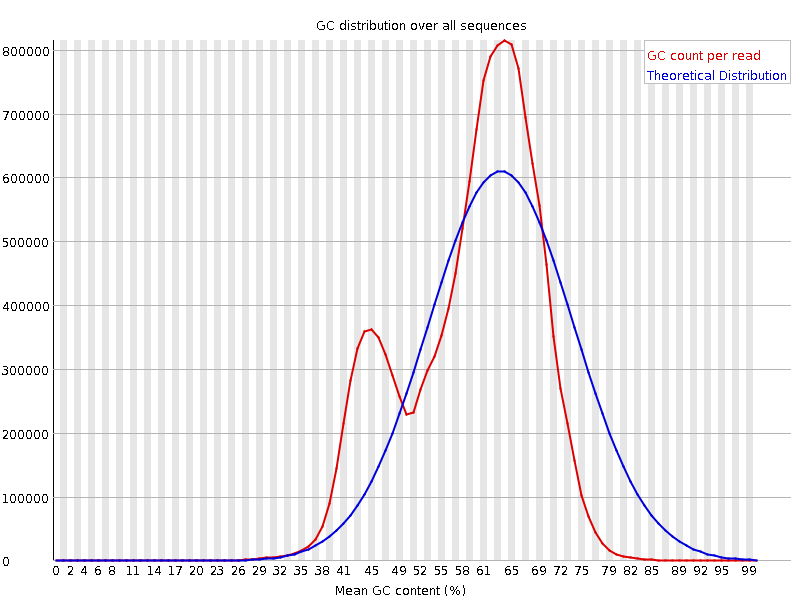
\includegraphics[width=\textwidth]{gccountexample.png}
    \caption{Example plot of the Light1\_9 showing the characteristic bimodal GC distribution of these libraries}
    \label{fig:gc}
\end{figure}

\subsubsection{Assembly and assembly assessment}

While an attempt can be made to identify optimal pre-processing
parameters using heuristic measures like mapping metrics against a reference. 
It is very difficult to identify the parameters (preprocessing or otherwise) which will leads to the ``best'' 
\textit{de novo} assembly prior to actually generating the assembly.
  Assembly can be considered an example of Wolpert and Macready's ``No Free Lunch Theorems'' \citep{Wolpert1995,Wolpert1997} 
  as (in the case of \textit{de novo} assembly) it is fundamentally a hamiltonian/eulerian cycle search problem (equivalent
    in the de-Bruijn formulation) and therefore any two assembly implementations (in different assemblers and/or
    with different parameters) should ultimately be equivalent across all possible input datasets.\footnote{
    This should be taken with a pinch of salt, a proof of this theorem applied to the case of assembly is beyond
both the scope of this thesis and my abilities}.  For this reason, it is necessary to try
assembly using a random of assembly parameters and indeed a range of both \textit{de novo} and referenced assemblers. 
For this reason, 4 \textit{de novo} assemblers were used: Trinity, SOAPdenovo, TransAbyss, and Velvet/Oases (see \ref{sec:methods} for details)
as well as Cufflinks/TopHat2/Bowtie2 for referenced assemblies.  However, as Trinity overwhelming generated the best 
\textit{de novo} assemblies in preliminary assemblies the majority of optimisation focussed on this assembler.


Unfortunately, the task of identifying the ``best'' \textit{de novo} transcriptome assembly is also a non-trivial 
task \citep{Neil2013}.  Many widely used assembly assessment metrics have been shown to be
inconsistent measures in simulated sequencing data, especially those metrics related to invidual
contigs (theoretically different transcript splices).  Metrics such as average length and N50
prove consistent across both simulated sequencing depth and read lengths i.e. they improve 
towards \citep{Neil2013}.  Furthermore, the number of possible metrics is greatly reduced
if assessment is mainly conducted in a reference-free manner \citep{Li2014}.  As the majority of
assemblies were \textit{de novo} and the suitability of the related but divergent genomes
as references was one area that was being investigated it was necessary to restrict to reference-free
assembly assessments.  Therefore, a model-based reference-free assembly scoring algorithm (RSEM-EVAL \citep{Li2014} was,
    along with standard (if imperfect) metrics, used to evaluate different assemblies. 


\subsection{Binning}

However, even once a good assembly has been generated it is still necessary to identify the likely
originating species of a given transcript i.e. host, endosymbiont, food bacterial contaminant or other
contaminant.  While a successful partitioned pre-assembly strategy may simplify this process it would still
be sensible to confirm bins using downstream analyses that use full length assembled transcripts and thus
more potential data than are present in shorter individual PE reads.  Rough, approximate bins were
generated using a simple "top BLAST hit" approach following ORF calling (using Tetrahymena and Universal
encodings) against a set of representative predicted proteomes.  In order to assess how accurate these
bins were likely to be, 10,000 were randomly selected and rapid maximimum-likelihood phylogenies were
generated using the transcript sequence as a seed to sample the entire RefSeq protein nr database.
This was accomplished using ``Dendrogenous'', a rewritten and modified version of a pipeline originally known 
as ``Darren's Orchard'' which first appeared in \citep{Richards2009g}.  Phylogenies were manually assessed to check
whether the resultant topology was congruent with the BLAST based binning i.e. are supposedly ``endosymbiont''
transcripts branching principally with archaeplastida taxa.  
However, due to the slow largely manual nature of this phylogeny assessment process it would be infeasible
to repeat this for all transcripts generated from a single assembly, let alone investigating several. 

Therefore, this became a fundamental classification problem with the 10,000 manually verified phylogenies
forming a handy training dataset for supervised learning.   To determine the best performing
classification algorithm and hyperparameters for this dataset an automated search was conducted 
using bayesian optimisation.  This was then converted to a binning script named ``Arboretum''.



%%Can you separate transcripts from host, endosymbiont and food bacteria?
%Current practices and how they were applied - BLAST, GC etc
%Initial binning vs phylogenetics - seems better
%But still too work intensive - use manually done 10,000 for rest of transcriptome therefore ML
%Flowchart of tool 
%t-SNE plot of vectors
%classifier log-loss and learning curve comparison using logistic regression, SVM with diff kernels
%Convergence check for SVM hyperparameters
%anomaly detection?
%
%Transcriptome Assembly:
%
%- Trimming: MacManes 5, 30 (also did 12 and 35)
%- Error correction: Spades error correction
%- GC clustering parKour
\section{Methods} 

\subsection{Sample Preparation and Sequencing}

\subsubsection{Bulk transcriptomic RNA preparation}
For bulk transcriptomic analyses CCAP 1660/12 cells were harvested in a way to minimise the 
number of bacterial prey species from the culture, \textasciitilde \(10^{6}\) 
cell aliquots were strained through \(40\mu m\) sieves, filtered on 
\(10 \mu m\) nylon filters, 
before finally being filtered on \(8 \mu m\) TETP polycarbonate filters using a 
low-pressure filtration pump.  Collected samples were either immediately 
quick-frozen in liquid nitrogen for storage (\(-20\)\celsius for short-term storage 
and \(-80\)\celsius for longer storage) or harvested by centrifugation.  
In order to investigate the two main metabolic states of the symbiosis 
(i.e. under light conditions during active photosynthesis and in the dark 
when no photosynthesis is taking place) samples were extracted 5 hours into 
the light and dark phase of the 12:12 hour day-night cycle.

To ensure extracted RNA was representative of healthy and interacting host 
and endosymbionts care was taken to minimise the number of dead/dying cells 
from which RNA was extracted.  In order to do this, a subsample was taken 
from each culture during the process of harvesting and scored for dead/dying cells.  
Cell assays were formed by taking 1-2ml of each harvest cell pellet and 
fixed using 40\(\mu l\) Lugol's solution (0.5g \(I_{2}\) and 1g KCl in 8.5ml 
of MilliQ water). Dead/dying cells were identified as broken or puckered cells 
and counted using light microscopy.  Samples containing >10\% dead/dying cells 
were discarded and no RNA extracted from them.

In order to lyse collected samples, cells were washed from the filter or the 
pellet was resuspended in 1ml TriReagent (Sigma) heated to \(60\)\celsius. 
Cells were vortexed with sterile \(300\mu m\) glass-beads for 15s, incubated at 
room temperature for 10 minute, vortexed for 15s, quick-frozen in liquid 
nitrogen and stored at \(-20^{o}C\) before further processing.  
Samples were defrosted, vortexed for 15s, placed in a heat-block set 
to \(60^{o}C\) for 10 minutes while continuing to be vortexed, removed from 
heating and vortexed again for 15s.  
RNA was extracted by adding 0.2ml of Chloroform to the glass-bead-trizol-sample 
solution, shaking for 15s, incubating for 5 minutes at room temperature and 
centrifuging at 12,000g for 15 minutes at $4^{o}$C.  
The upper-phase was then transferred to an RNAse-free 1.5ml tube and an 
equal volume (\textasciitilde$0.5$ml) of isopropanol was added before shaking for 15s.  
The isolated RNA was then incubated at $-20^{o}$C for 10 minutes 
(up to several hours) before being collected as a pellet using a centrifuge at 
10,000g for 10 minutes at $4^{o}$C (supernatant was discarded). 
The RNA pellet was then washed with 1ml of 75\% ethanol and centrifuged 
twice at 10,000g for 10 minutes at $4^{o}$C with the supernatant being 
discarded after each centrifugation.  
Pellet was dried before being resuspended in 100$\mu l$ of RNAse-free water.  
The RNA was then cleaned further using the Qiagen RNeasy clean-up kit 
before being assessed for quality using ND-1000 (NanoDrop) and BioAnalyzer (Agilent).


\subsubsection{Single Cell RNA preparation}

For single cell transcriptomics, a ``cell-picking'' approach was used in which
\textit{P. bursaria} cells (from the CCAP1660/12 culture) were inspected on an inverted light microscope 
before being picked using an orally aspirated drawn-glass Pasteur pipette \citep{Garcia-Cuetos2012}.
In order to mininmise contamination from food bacteria present in the media these picked cells
were washed 3 times by serial transfer to \(10\mu l\) droplets of sterile NCL media.
The washed cell was then transferred to a \(10\mu l\) droplet of sterile water.
3 cells were picked 5 hours into both the lit and dark phase of the 12:12 hour day-night cycle.

Cells were transferred from their respective \(10\mu l\) droplets of sterile water to
a PCR tube containing \(6\mu l\) water and \(4\mu l \) lysis buffer (from the Qiagen
REPLI-g WTA Single Cell Kit) \citep{Korfhage2015}. To disrupt the cell beads (Sigma, \(425-600\mu m\), acid-washed)
were added to the meniscus, before submersion in liquid nitrogen for 5 seconds.  The sample was 
then thawed before vortexing for 1 minute.  
mRNA was selectively amplified and reverse transcribed to cDNA using poly-A selection.  The cDNA
was then amplified using multiple displacement amplification and the amplified cDNA purified
using a QIAamp DNA mini kit eluted in \(100\mu l\) elution buffer.

Subsequently, this process was repeated for a further 5 dark samples.

%\subsubsection{Single Cell genomic DNA preparation}
%Cells were transferred from their respective \(10\mu l\) droplets of sterile water to a microncentrifuge tube.
%CTAB method adapted from \citep{Winnepenninckx1993}.  Cells were disrupted by vortexing for 5 minutes with
%\(748.5\mu l\) CTAB extraction buffer (at 37\celsius) and ceramic beads (Sigma, \(425-600\mu m\), acid-washed).
%The tube was then incubated for 50 minutes at 37\celsius, vortexed for 5 minutes, and incubated for a further 50
%minutes at 60\celsius. DNA was extracted 3 times using phenol, chloroform and isoamylalcohol at a 25:24:1 ratio (pH 8),
%washed with 70\% ethanol and re-suspended in \(2.5\mu l\) TE buffer (pH 8). This DNA then underwent 
%Multiple displacement-based whole genome amplification using the Repli-G Single Cell Kit before purification using a 
%QIAmp DNA mini kit before elution in \(100\mu l\) elution buffer.  

\subsubsection{Library preparation}

For both bulk and single cell preparations each cDNA sample was fragmented in \(130\mu l\) 1xTE buffer on the Covaris E220 
with a target size of \(225bp\) (duty factor of \(10\%\), 200 cycles per burst, peak incident power
of 175, \(200s\) at \(7^{o}C\)). Fragment sizes were checked on a BioAnalyzer (Agilent) 7500 DNA chip.
cDNA was then concentrated using a GeneRead kit column with a elution in \(35\mu l\). Fragmentation
step was then repeated 3 times (\(110s\)) until majority of cDNA in each library was between \(200-250bp\)

cDNA ends were then end-repaired, adenylated and adapters ligated using the NEXTFlex (Biooscientfic) sequencing kit 
according to the manufacturer's instructions and using NEBNext (New England Biolabs) indices.  Also following
the NEXTFlex kit instructions, MgNa bead purification was done before and after PCR amplification using
NEBNext reagents.  Finally, prepared libraries were size selected using a Blue Pippin machine at a size selection
of \(350bp\) (range \(315-385bp\)).

A final bioanalyzer step was conducted with individual library concentrations ranging from \(0.66-4.09nM\).

\subsubsection{Sequencing}

The bulk day and night library were paired-end \(76bp\) sequenced using an Illumina Genome
Analyzer II by the Exeter University Sequencing Service.  The two libraries were sequenced
on separate flowcells.

Single cell libraries were paired-end \(150bp\) using an Illumina HiSeq 2500 by Exeter
Sequencing Service. 3 dark and 3 light samples were sequenced multiplexed on a single 
flowcell lane.  The 5 additional dark samples were later sequenced multiplexed on a single
flowcell lane.

\subsubsection{Baseline bulk assembly}

A ``baseline'' assembly was completed of the bulk RNA-Seq libraries so that there was a fixed
means of comparison against which the most effective means of incorporating single cell
sequencing data could be incorporated.

Adapters and bases <Q20 were trimmed from these bulk reads by the Exeter Sequencing Service
using Fastq-MCF \citep{Aronesty2013} and assembled using the 4 available \textit{de novo} 
transcriptome assembly tools with their default settings: SOAPdenovo-Trans \citep{Xie2014}, 
Trans-ABySS \citep{Robertson2010}, Trinity \citep{Haas2013} and Velvet/Oases \citep{Schulz2012a}

Resultant assemblies were then compared using standard assembly statistics and the reference
free probabilistic assembly assessment RSEM-EVAL package (part of DETONATE) \citep{Li2014}.
Using these metrics a single assembler and assembly was selected for further downstream
analysis including incorporation of single-cell libraries.

\subsection{Library Screening}

To investigate contamination and the taxonomic profile of sequenced single cell libraries 
the ``DueyDrop'' tool was developed.  

Briefly, for each single cell library 5 batches of 10,000 PE reads were sampled 
using the reservoir sampler \citep{Vitter1985} implemented in Heng Li's seqtk library \citep{SeqtkGitHub}.
Despite 5 batches of 10,000 reads theoretically being equivalent to 50,000 random samples by splitting
sampling and using a different random seed any problems from poor randomisation implementation 
was minimised and consistency of taxonomic profiles could be easily assessed.
These randomly sampled reads were subsequently aligned to NCBI's Protein NR RefSeq database \citep{Pruitt2007}
using the efficient short-read optimised BLASTX implementation of DIAMOND \citep{Buchfink2015} (at a expectation
    of \(e^{-5}\) and top hits for each read retained.  Gene identifiers (GI) were extracted from these tops hits and queried against a
local copy of the NCBI taxonomy database \citep{Federhen2012} to recover a hit taxonomic lineage for each
read that aligned to a sequence within NR database. These lineages were then interactively tallied 
at several different taxonomic levels (e.g. domain level - eukaryote vs bacteria, or lower level - viridiplantae vs ciliate) and variances
calculated.  Results were then tabulated and libraries compared to assess whether any libraries appeared
abberrant.

Scripts used to conduct this are available in my thesis scripts github repository:
\url{https://github.com/fmaguire/dueydrop}

\subsection{Trimming optimisation}

To investigate optimal trimming for single cell libraries a naive grid search across trimming parameters was used.
Specifically, 5000 PE reads were randomly sampled without replacement from each of the raw FASTQ libraries 
using the streaming reservoir sampling \citep{Vitter1985} algorithm implemented in Heng Li's 
seqtk C library (\citep{SeqtkGitHub}).
To guarantee the pairing was maintained the same random seed was used for the left and right read
of each library. This seed was subsequently incremented with each library sampled.
These random samples were subsequently trimmed using a variety of parameter values and combinations therein 
(see \ref{table:parameters} for details).
The trimmed samples were then mapped to the ``baseline'' bulk RNA-Seq transcriptome reference dataset using bowtie2
\citep{Langmead2012} with maximum and minimum insert sizes of 37bp and 1161bp (derived from library preparation
fragment size distribution and histrogram of mapped insert sizes for untrimmed reads against bulk reference).
For each set of trimming parameters the following bowtie2 mapping statistics were recorded: 
\begin{itemize}
    \item number of paired reads uniquely mapping in a paired 
fashion (concordantly exactly 1 time), 
    \item number of paired reads which uniquely mapped 
singly (discordantly exactly 1 time), 
    \item the total number of reads which survived trimming.
\end{itemize}

These values were assessed in comparison to the ``null mapping'' i.e. these same mapping statistics for the same
randomly sample reads for each library but this time entirely untrimmed.  

%Therefore, if \(i\) represents the SCT library being sampled and \(j\) represents the number of random samples of
%5000 PE reads from each library, then a function \(f\) which applies trimming with a given set of a 
%paramaters \(\theta\) and returns a weighted sum of the mapping statistics can be defined as follows with
%weights defined by our priorities:
%
%\[
%    f(x_{ij}, \theta) = map_{\theta,concord} + \frac{1}{2} * map_{\theta,discord} + \frac{1}{4} * survive_{\theta} 
%
%\]
%
%Specifically, we are particularly interested in maximising the number of reads which congruently map to the baseline
%bulk assembly.  
%
%
%Therefore, the optimal trimming paramters \theta are those which maximise the following cost function
%
%\[
%    J(\theta) = \sum^{I}_{i=0} \sum^{J}_{j=0} f(x_{ij}, \theta) - f(x_{ij}, \emptyset)
%\]

We are particularly interested in determing the trimming parameters which maximise the raw number of reads mapping rather than
the proportion, as a harsh trim may generate a high proportion of mapping reads due to spuriously discarding 
many reads.  

Different trimming tools were also compared to attempt to determine the optimal tool.
This will be discussed and explained in the results/discussion section, however Trimmomatic \citep{Bolger2014a}
was chosen for targeted trimming parameter optimisation.

To that end a gridsearch was conducted over a sliding window trim of size 5, 10 
with mininum quality score of 5, 10, 20, 25, and 30 in Trimmomatic.  Additionally, 
a head and tail crop of 5 was used, and adapters trimming parameters
ranged from seed mismatch of 2, 4, palindrome clip thresholds of 20 and 30, 
and a simple clip threshold of 10, 15 and 20 in Trimmomatic's ILLUMINACLIP setting.

Scripts used to conduct this are available in my thesis scripts github repository:
\url{https://github.com/fmaguire/thesis_scripts/tree/master/chapter_2_assembly_and_binning/trimming_optimisation}

\subsection{Error correction}

The effect of error correction on assemblies involving single cell libraries was assessed 
by applying two different error correction algorithms. 

Firstly, trimmed and taxonomically selected libraries were error corrected using the
Bayeshammer \citep{Nikolenko2013} based approach implemented as part of the Spades single-cell  
genome assembler \citep{Bankevich2012}.

Additionally, an RNA-Seq (but not scRNA-Seq) error correction tool ``SEECER'' \citep{Le2013} was 
applied to trimmed bulk and single cell reads.

The impact of each of these error correction algorithms at the read level was assessed as well 
as their subsequent impact on downstream assembly metrics, particularly RSEM-EVAL likelihood.


\subsection{GC Partitioning of Reads}

To assess the utility of pre-assembly read partitioning an unsupervised clustering tool was created:
Paired Arrangement of Reads via K-means On Unlabelled Reads (parKour).
This C++ tool implements a fast and efficient K-means clustering of reads based on the dual features
of GC\% in forward and reverse paired reads.

Specifically, parKour:
\begin{enumerate}
    \item Parse user input of paired FASTQ files corresponding to Forward and Reverse Paired-End reads, and desired number of clusters
    \item Simultaneously iterate over the pair of FASTQ files calculating the GC\% for each loading results into an Armadillo \(2xN\) matrix \citep{Sanderson2010} where \(N\) is the total number of PE reads
    \item Bradley-Fayyad K-means \citep{Bradley1998} clustering as implemented in the MLPACK library \citep{mlpack2013}
    \item Re-read the two input FASTQs assigning them to output files based on the assigned cluster of the pair
\end{enumerate}

GNUplot \citep{Gnuplot_4.4} was used to visualise classification and cluster assignment.
This approach was attempted using a range of expected clusters from 2 to 5.

Scripts used to conduct this are available in a github repository:
\url{https://github.com/fmaguire/parKour}


\subsection{Assembly}

Trimmed bulk and taxonomically selected single cell libraries
were mapped to \textit{Chlorella} NC64A, \textit{Coccomyxa C169}, 
\textit{Tetrahymena thermophila} and \textit{Paramecium caudatum} MAC genomes.
The former pair being the closest available genomes to the endosymbiont and the latter to the host.

Mapping was done using the TopHat2 spliced aligner \citep{Kim2013} against
the genomes and was supplemented with and without annotated ORF information (in the form of gtf).
GTF files were generated from best avaiable gene annotations in the form of GFF files using gffread (part of
cufflinks).
Cufflinks \citep{Trapnell2011} was then used to extract isoforms from the spliced alignments.


For \textit{de novo} assembly, assemblies were conducted using Trinity \citep{Grabherr2011}, 
SOAPdenovo-Trans \citep{Xie2014}, TransAbyss \citep{Robertson2010} and Velvet/Oases \citep{Schulz2012}.
However, as Trinity overwhelming generated the best assemblies i.e. recovered the same trancripts
but generally longer and more accurately collapsed into different isoforms, Trinity was 
used for all further downstream optimisation.


ORFs were called from assembled transcripts using transdecoder \citep{Haas2013} with 
a minimum protein size of 100aa.  \textit{Paramecium} uses an alternative
genetic code in which two universal stop codons (UAA, UAG) are reassigned to glutamine.
Due to this all ORFs were initially called using this encoding for initial binning
purposes as spuriously extended transcripts were favourable to falsely truncated
ones.  

%After assembly transcripts shorter than 200bp were removed and CD-HIT was sued to elimiate small 
%transcripts with 99\% idendity to longer transcripts  ``cd-hit-est -i TREANSCRIT -c 0.99 -o Ol:UTPU''

\subsection{Binning}

\subsubsection{Initial bins}

Initially, 10,000 randomly chosen transcripts were binned into their predicted source - 
Host (H), Unknown but likely Host (U(H)), Endosymbiont (E), Unknown but likely Endosymbiont (U(E)), Food (F), Unknown but likely Food (U(F)), and
Unknown (U). 
Each of the assembled transcripts were BLASTed against a database consisting of the following predicted proteomes: 
\textit{Chlorella} NC64A, \textit{Chlamydomonas reinhardtii}, \textit{Coccomyxa} C169,
\textit{Paramecium tetraurelia}, \textit{Tetrahymena thermophila}, \textit{Arabidopsis thaliana}, \textit{Homo sapiens} (help-
    ing to identify contamination), \textit{Saccharomyces cerevisiae}, \textit{Schizosaccharomyces pombe}, \textit{Bacillus
cereus} ATCC 14579, \textit{Escherichia coli} 536, \textit{Escherichia coli} O157 H-7, \textit{Salmonella typhimurium}
LT2 and \textit{Escherichia coli} K-12 (the last 5 genome datasets helping to identify food bacterial
genes). Then initial bins were classified as follows:
\begin{itemize}
    \item Endosymbiont (E): Transcript’s highest scoring BLAST hit at \(-50E\) was to Coccomyxa,
        Chlamydomonas or Chlorella. Or transcript’s highest scoring hit at \(-20E\) was one of those
species and the longest likely coding region in the transcript was using the universal codon
table.
\item Unknown but likely Endosymbiont (U(E)): \(-10E\) hit to Coccomyxa, Chlamydomonas or
Chlorella and longest likely coding region was using the universal codon table. Or tran
script’s highest hits at \(-10E\) and \(-20E\) were to one of those genomes regardless of coding
region presence.
\item Host (H): Transcript’s highest hits at \(-50E\) were to Paramecium tetraurelia or Tetrahymena
    thermophila. Or highest hit at \(-20E\) was one of those species and longest likely coding
region was using the Tetrahymena codon table.
\item Unknown but likely Host (U(H)): \(-10E\) hit to Paramecium tetraurelia or Tetrahymena
thermophila and longest likely coding region was was using the Tetrahymena codon table.
Or transcript’s highest hits at \(-10E\) and \(-20E\) were to one of those genomes regardless of
coding region presence.
\item Food (F): Transcript’s highest scoring BLAST hit at \(-50E\) was to one of the E. coli species
    or Salmonella. Or transcript’s highest scoring hit at \(-20E\) was one of those species and
the longest likely coding region in the transcript was using the universal codon table.
\item Unknown but likely Food (U(F)): \(-10E\) hit to one of the E. coli species or Salmonella and
longest likely coding region was using the universal codon table. Or transcript’s highest
hits at \(-10E\) and \(-20E\) were to one of those genomes regardless of coding region presence.
\item Unknown (U): highest scoring hits to Arabidopsis, Homo sapiens, Saccharomyces or Schizosac-
charomyces or any sequence not fitting into the above categories.
\end{itemize}


\subsubsection{Dendrogenous}

To rapidly generate phylogenies an established lab tree generation pipeline, known as ``Darren's Orchard'' 
\citep{Richards2009g} was modified and converted to python3.  This new pipeline ``Dendrogenous'' 
takes in a multi-fasta set of inputs and a set of genomes to search against.
For each input sequence:
\begin{enumerate} 
    \item The specified genome database is queried using BLASTP
    \item The results are parsed and a fasta file of putative homologues is created, with inputs that have fewer than a specified 
        number of hits (default of 5) ejected.
    \item A multiple sequence alignment (MSA) is created from this fasta using Kalign (chosen for its speed) \citep{Lassmann2009}
    \item This MSA is then masked automatically to remove ambiguous sites using TrimAL \citep{Capella-Gutierrez2009} and masked alignments
        with fewer than a specified number of sites (default of 30) are ejected from the pipeline.
    \item A rapid maximum-likelihood phylogenetic tree is generated using FastTree2 \citep{Price2010}
    \item Finally, encoded taxonomic information is recovered from the ``cider'' database of the original ``Darren's Orchard'' pipeline 
        and the trees are named with full species names.
\end{enumerate}
The two key improvements are that of full and efficient parallelisation of the tree generation process (see \ref{fig:ddg})
and increased use of filestreams to pass data between pipeline stages.  This latter modification reduces costly and slowly
file reading and writing operations.

In the process of creating this modified phylogenetic pipeline I upgraded the general purpose python phylogenetic toolkit
ETE \citep{Huerta-Cepas2010} to support python3.  As ETE is an open source project I submitted these changes
to the maintainer and they have subsequently been merged into the master.  These changes compose a significant proportion of
the latest major release version of this toolkit \url{https://github.com/jhcepas/ete/pull/105}.

\begin{figure}
    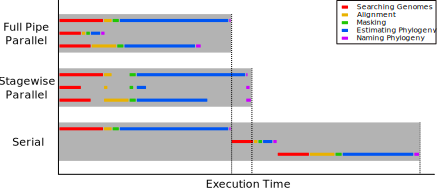
\includegraphics[width=\textwidth]{dendrogenous_parallel.pdf}
    \caption{A explanatory plot showing 3 different possible architectures for a tree generation pipeline. 
        Serial, in which each phylogeny is run one after another.  This form makes no use of multiprocessing
        facilities, however, a moderate but significant performance improvement can be achieved by allowing
        each stage in the pipeline to utilise multiple cores i.e. the trees are generated serially but during
        their generation alignment and blasting making use of multiple processors.          
        Stagewise parallel, where for example, all alignments for each input sequence are run side-by-side 
        and masking begins once the last sequence has finished alignment.  The disadvantage of this is a single
        slow stage for one input sequence can hold up the whole pipeline and leave resources idle.  Additionally,
        by running many of the same type of process at the same time, each with similar resource requirements,
        the risk of hardware bottlenecking is increased compared to a more heterogenous load.
        Finally, fully parallel runs each input sequence through the pipeline stage-by-stage separately
    from all other inputs to the pipeline. This prevents blocking and allows efficient using of resources.}
    \label{fig:ddg}
\end{figure}

40 genomes covering the diversity of the tree of life, with a particular focus on green algal and ciliate representatives 
were selected for this phylogenetic generation.
\begin{itemize}
    \item \textit{Arabidopsis thaliana}
    \item \textit{Chlamydomonas reinhardtii }
    \item \textit{Ostreococcus tauri}
    \item \textit{Micromonas pusilla CCMP1545}
    \item \textit{Chlorella variabilis NC64A}
    \item \textit{Chlorella vulgaris C-169}
    \item \textit{Physcomitrella patens}
    \item \textit{Saccharomyces cerevisiae S288C}
    \item \textit{Neurospora crassa OR74A}
    \item \textit{Homo sapiens}
    \item \textit{Mus musculus}
    \item \textit{Dictyostelium discoideum}
    \item \textit{Paramecium caudatum}
    \item \textit{Paramecium tetraurelia}
    \item \textit{Tetrahymena thermophila macronucleus}
    \item \textit{Oxytricha trifallax}
    \item \textit{Toxoplasma gondii}
    \item \textit{Guillardia theta}
    \item \textit{Bigelowiella natans}
    \item \textit{Emiliania huxleyi CCMP1516 }
    \item \textit{Aureococcus anophagefferens}
    \item \textit{Ectocarpus siliculosus}
    \item \textit{Schizosaccharomyces pombe}
    \item \textit{Bacillus cereus ATCC 14579}
    \item \textit{Escherichia coli str. K-12 substr. MG1655}
    \item \textit{Escherichia coli O157 H7 str. Sakai}
    \item \textit{Salmonella enterica subsp. enterica serovar Typhi str. CT18}
    \item \textit{Amycolatopsis mediterranei U32}
    \item \textit{Aquifex aeolicus VF5}
    \item \textit{Borrelia burgdorferi B31}
    \item \textit{Chlamydophila pneumoniae CWL029}
    \item \textit{Chlorobium tepidum TLS}
    \item \textit{Deinococcus radiodurans R1}
    \item \textit{Caulobacter crescentus CB15}
    \item \textit{Sulfolobus islandicus M.14.25}
    \item \textit{Nanoarchaeum equitans Kin4-M}
    \item \textit{Haloferax mediterranei ATCC 33500}
    \item \textit{Methanococcus maripaludis S2}
    \item \textit{Cenarchaeum symbiosum A}
\end{itemize}

10,000 transcripts from the initial BLAST based bins were used to generate phylogenies 
and were manually parsed and assessed for phylogenetic congruence with their bin.
For example, do host binned sequences predominantly branch with other ciliate sequences?
Do endosymbiont binned sequences mainly branch with archaeplastida sequences. 


\subsubsection{Arboretum}

Using these 10,000 manually verified phylogenetic bins as a training dataset a supervised classification
script ``Arboretum'' was created.  The cardinalities of this training set are relatively balanced, all within
the same order of magnitude 1975 endosymbiont phylogenies, 2600 host, 3456 food, and 1969
unknown. 


``Arboretum'' parses phylogenies and identifies the k (default of 10) nearest branches to the seed transcript
the phylogeny was generated from.  The species of these closest leaves is queried taxonomically using the
NCBI taxonomy local database implemented in the ETE toolkit.  With a set of look-up filters e.g.
sequences from ciliates can be defined as "host-like", a set of vectors is created for each phylogeny.  
These are N-dimensional vectors where N is the number of class labels being used. 
For example, in this specific case: "endosymbiont", "host", "food/bacterial", and "unknown".
The magnitude of each dimension is the summed reciprocal phylogenetic distance between the root node and all
of the nearest branches that have been identified as being indicative of a certain class.

1,000 vectors from this training set were held out to form the test set and all models were then trained
using stratified 5-fold cross-validation on the remaining 9,000 training vectors. 
Support vector machines, random forest and logistic regression algorithms as implemented in scikit-learn 
were evaluated for performance manually and best performing classification algorithm was selected.
Additionally, an autoML method in which all available models are considered as hyperparameters in an efficient
bayesian optimisation approach was also attempted \citep{Komer2014}. 
Model performance was evaluated using a weighted average of all against one f1-scores.

\section{Results and Discussion} 

\subsection{Library selection}
% negatives ??
Using ``DueyDrop'' the taxonomic profile of each library was determined (see \ref{tab:sct_duey}).
Profiling raw vs trimmed reads made a fraction of a percent of difference in terms of the resultant taxonomic profile. Therefore, all 
shown data is derived from raw profiles (with the exception of the bulk profiles).

\begin{table}[h]
     \begin{tabular}{@{}|l|l|l|l|l|l|l|l|@{}}
         \cmidrule(r){1-6} \cmidrule(l){8-8}
         \textbf{SCT Library} & \textit{\textbf{PE}} & \textbf{Eukaryote} & \textbf{Bacteria} & \textbf{Alveolate} & \textbf{Viridiplantae} &  & \textbf{Total Hits} \\ \cmidrule(r){1-6} \cmidrule(l){8-8} 
         \textit{Light1-9}    & \textit{R1}          & 51.89 +/- 0.45     & 9.37 +/- 0.26     & 25.15 +/-  0.71    & 7.45 +/- 0.33          &  & 69.49 +/- 0.37      \\ \cmidrule(lr){2-2}
                              & \textit{R2}          & 51.75 +/- 0.25     & 8.82 +/- 0.24     & 24.85 +/- 0.56     & 7.49 +/- 0.21          &  & 68.75 +/- 0.29      \\ \cmidrule(r){1-6} \cmidrule(l){8-8} 
         \textit{Light1-10}   & \textit{R1}          & 46.35 +/- 0.56     & 15.72 +/- 0.46    & 22.96 +/- 0.24     & 6.94 +/- 0.26          &  & 68.73 +/- 0.30      \\ \cmidrule(lr){2-2}
                              & \textit{R2}          & 46.12 +/- 0.83     & 15.14 +/- 0.48    & 23.13 +/- 0.38     & 6.99 +/- 0.37          &  & 68.73 +/- 0.30      \\ \cmidrule(r){1-6} \cmidrule(l){8-8} 
         \textit{Light1-11}   & \textit{R1}          & 58.28 +/- 0.47     & 3.62 +/- 0.12     & 28.68 +/- 0.43     & 8.20 +/- 0.40          &  & 71.38 +/- 0.49      \\ \cmidrule(lr){2-2}
                              & \textit{R2}          & 57.74 +/- 0.27     & 3.50 +/- 0.10     & 28.23 +/- 0.36     & 8.41 +/- 0.31          &  & 70.42 +/- 0.20      \\ \cmidrule(r){1-6} \cmidrule(l){8-8} 
         \textit{Dark1-2}     & \textit{R1}          & 28.64 +/- 0.51     & 22.88 +/- 0.61    & 12.23 +/- 0.28     & 4.93 +/- 0.19          &  & 60.31 +/- 0.49      \\ \cmidrule(lr){2-2}
                              & \textit{R2}          & 28.29 +/- 0.24     & 21.06 +/- 0.21    & 12.13 +/- 0.28     & 4.87 +/- 0.34          &  & 57.65 +/- 0.35      \\ \cmidrule(r){1-6} \cmidrule(l){8-8} 
         \textit{Dark1-3}     & \textit{R1}          & 9.48 +/- 0.43      & 25.07 +/- 0.42    & 2.15 +/- 0.13      & 2.60 +/- 0.27          &  & 41.43 +/- 0.68      \\ \cmidrule(lr){2-2}
                              & \textit{R2}          & 8.89 +/- 0.19      & 23.11 +/- 0.52    & 2.13 +/- 0.16      & 2.45 +/- 0.18          &  & 38.50 +/- 0.46      \\ \cmidrule(r){1-6} \cmidrule(l){8-8} 
         \textit{Dark1-5}     & \textit{R1}          & 5.56 +/- 0.19      & 23.99 +/- 0.44    & 1.07 +/- 0.07      & 2.89 +/- 0.11          &  & 36.72 +/- 0.33      \\ \cmidrule(lr){2-2}
                              & \textit{R2}          & 4.94 +/- 0.21      & 21.75 +/- 0.53    & 1.02 +/- 0.11      & 2.33 +/- 0.17          &  & 33.06 +/- 0.52      \\ \cmidrule(r){1-6} \cmidrule(l){8-8} 
         \textit{Dark2-2}     & \textit{R1}          & 12.32 +/- 0.25     & 9.81 +/- 0.19     & 3.73 +/- 0.16      & 4.33 +/- 0.17          &  & 27.65 +/- 0.47      \\ \cmidrule(lr){2-2}
                              & \textit{R2}          & 11.53 +/- 0.15     & 9.00 +/- 0.17     & 3.67 +/- 0.22      & 3.74 +/- 0.12          &  & 25.71 +/- 0.39      \\ \cmidrule(r){1-6} \cmidrule(l){8-8} 
         \textit{Dark2-3}     & \textit{R1}          & 32.07 +/- 0.31     & 7.43 +/- 0.15     & 12.81 +/- 0.21     & 4.71 +/- 0.21          &  & 48.42 +/- 0.53      \\ \cmidrule(lr){2-2}
                              & \textit{R2}          & 32.47 +/- 0.24     & 6.68 +/- 0.21     & 13.11 +/- 0.43     & 4.58 +/- 0.12          &  & 47.92 +/- 0.28      \\ \cmidrule(r){1-6} \cmidrule(l){8-8} 
         \textit{Dark2-6}     & \textit{R1}          & 24.11 +/- 0.28     & 8.55 +/- 0.11     & 9.04 +/- 0.35      & 5.27 +/- 0.15          &  & 41.69 +/- 0.45      \\ \cmidrule(lr){2-2}
                              & \textit{R2}          & 22.89 +/- 0.55     & 7.44 +/- 0.17     & 8.74 +/- 0.49      & 4.36 +/- 0.24          &  & 38.85 +/- 0.58      \\ \cmidrule(r){1-6} \cmidrule(l){8-8} 
         \textit{Dark2-7}     & \textit{R1}          & 9.96 +/- 0.24      & 16.89 +/- 0.27    & 4.22 +/- 0.24      & 2.83 +/- 0.17          &  & 37.06 +/- 0.40      \\ \cmidrule(lr){2-2}
                              & \textit{R2}          & 8.77 +/- 0.18      & 15.00 +/- 0.43    & 3.94 +/- 0.14      & 2.16 +/- 0.11          &  & 32.86 +/- 0.29      \\ \cmidrule(r){1-6} \cmidrule(l){8-8} 
         \textit{Dark2-8}     & \textit{R1}          & 28.24 +/- 0.48     & 4.45 +/- 0.13     & 12.00 +/- 0.32     & 4.69 +/- 0.06          &  & 40.50 +/- 0.37      \\ \cmidrule(lr){2-2}
                              & \textit{R2}          & 28.22 +/- 0.47     & 4.30 +/- 0.22     & 11.98 +/- 0.37     & 4.32 +/- 0.24          &  & 40.05 +/- 0.22      \\ \cmidrule(r){1-6} \cmidrule(l){8-8} 
     \end{tabular}
     \caption{Taxonomic profiles of raw single cell libraries. All values are percentage of reads mapping to that category +/- the standard deviation between sample replicates}
 \label{tab:sct_duey}
\end{table}

Using this approach we identified and discarded Dark1-3 Dark1-5 Dark2-2, and Dark 2-7 as likely contaminated, particularly noteworth is the incredibly
low proportion of sampled reads mapping to known alveolate (or even eukaryotic) sequences from these libraries.   
Interestingly, these samples didn't appear to be uniformly especially enriched for likely bacteria derived reads and we cannot say for certain whether they represent
``failed'' libraries in some way or merely a previously uncharacterised sub-population that is less transcriptionally active. 
Removal of these libraries halved the number of recovered transcripts in Trinity \textit{de novo} assemblies as can be seen in the the assembly
summaries below.

Despite evidence that nanoscale methods can greatly reduce levels of contamination \citep{Blainey2011}, the taxonomic profiling conducted here
indicates a high level of bacterial (and viral) contamination in the scRNA-Seq.  Intriguingly, similar taxonomic profiling of the bulk
libraries revealed a very low percentage of reads mapping to any sequence in the nr protein database.  This was significantly lower than the
sc-RNAseq libraries.  While this finding is concerning it is likely to be an artefact of the older sequencing platform the bulk data was generated on.
These paired reads were sequenced via the GAII and were half the length of the HiSeq2500 reads used for the SCTs.  Shorter reads and a relatively higher
technical error rate on this platform may have played a role in this marked decline in recognisable reads. 
Despite this the relative proportion of bacterial reads to eukaryote reads among the recognisable reads is much lower for bulk libraries than SCT.

This supports the findings of \citep{Kolisko2014}, in which enigmatic, bacterial contamination was a problem in single cell eukaryotic
transcriptomes.   One possible reason for this is that due to the high levels of amplification required, the poly-A selection step
in library prepartion is less effective at removing non-eukaryote mRNA transcripts.


Another, feature of the profiles of interest is the systematically low 
low levels of Viridiplantae related reads across both types of libraries and conditions.  The most likely culprit for
this is inefficiencies in the lytic step of RNA extraction for \textit{Micractinium} cells. 
Lysis is difficult in cells
with cell walls \citep{Korfhage2015} and \textit{Micractinium} is known for its robust chitin walls. 

Finally, both SCT and bulk dark libraries reflect a significantly lower proportion of eukaryote mapping reads. Either dark expressed transcripts 
reflect a high degree of novel, previously unsequenced, diversity, other uncharacterised contaminants are active at night or there is some aspect
of the extracted material in the dark that leads to problematic sequencing.  

%One potential explanation for this last scenario could be 
%an aggravated AT bias leading to high sequencing error due to a relatively greater proportion of AT-rich host derived reads 

\begin{table}[h]
     \begin{tabular}{@{}|l|l|l|l|l|l|l|l|@{}}
         \cmidrule(r){1-6} \cmidrule(l){8-8}
         \textbf{Bulk Library} & \textit{\textbf{PE}} & \textbf{Eukaryote} & \textbf{Bacteria} & \textbf{Alveolate} & \textbf{Viridiplantae} &  & \textbf{Total Hits} \\ \cmidrule(r){1-6} \cmidrule(l){8-8} 
         \textit{Light}    & \textit{R1}              &  9.66 +/- 1.55     & 0.18 +/- 0.13     &  6.28 +/- 1.41     &  0.86 +/- 0.3          &  &  10.10 +/- 1.48       \\ \cmidrule(lr){2-2}
                              & \textit{R2}           &  9.62 +/- 0.81     & 0.26 +/- 0.09    &  6.58 +/- 0.36     &  1.04 +/- 0.41         &  &  10.16 +/- 0.95      \\ \cmidrule(r){1-6} \cmidrule(l){8-8} 
         \textit{Dark}   & \textit{R1}                &  4.90 +/- 0.78     & 0.36 +/- 0.11    &  3.14 +/- 0.58     &  0.50 +/- 0.16        &  &  5.40 +/- 0.93      \\ \cmidrule(lr){2-2}
                              & \textit{R2}           &  5.50 +/- 1.25     & 0.22 +/- 0.19   &  3.82 +/- 0.81     &  0.50 +/- 0.12         &  &  6.02 +/- 1.22      \\ \cmidrule(r){1-6} \cmidrule(l){8-8} 
    \end{tabular}
    \caption{Taxonomic profile of the bulk transcriptome samples}
    \label{tab:bulk_duey}
\end{table}

``DueyDrop'' could potentially be improved in such a way that an entire library can be screened instead of just subsamples.
Briefly, this would involve quantifying exact k-mer matches between library reads and a pre-generated database of known taxa
using efficient probabilstic hashing datastructures such as a bloom filter, or more likely count-min sketch and an efficient
k-mer counting library such as Jellyfish \citep{Marcais2011}.  This would have a major speed advantage compared to the BLASTX-based method of ``dueydrop''
and would thus allow entire libraries to be checked in reasonable time.  However, it would require laborious workarounds to handle
k-mers shared between multiple taxa in the database, translation of reads and/or database sequences into a matching sense and form (e.g. protein),
and use of a locality-sensitive hash function to handle scenarios where there is no exact k-mer match. This latter issue is particularly
problematic for libraries consisting of transcripts from poorly sampled reaches of the tree of life where exact matches would become
commensuately rarer as sampling sparsity increases.  
While still affected by this problem, the BLASTX/Diamond approach implemented in the ``DueyDrop'' scripts are relatively more robust to these
problems due the explicit probabilistic modelling of sequence divergence built into the BLAST alignment algorithm (e.g. E-values).

Regardless, taxonomic profiling and contamination screening had great utility identifying potential problems in library preparation (e.g. chitin lysis) 
as well as offer a powerful means of removing problematic libraries from assembly.

\subsection{Assembly optimisation}

\subsubsection{Trimming}
While, there are many available tools for read-trimming (as discussed in \ref{ch:methods}) , 
Trimmomatic was my preferred tool as it maintains read-pair correspondence, is optimised for Illumina datasets and, allows user-defined ordering of trimming operations and can do adapter trimming \citep{Bolger2014a}.  
Furthermore, it has adequate (if not perfect) performance and is well documented.
However, other tools were also considered specifically Sickle \citep{JoshiGitHub}, FASTX-toolkit \citep{gordon2010fastx}, 
and cutadapt \citep{martin2011cutadapt}.

Sickle is an adaptive quality trimmer that has previously been used in single-cell transcriptome datasets 
from free-living eukaryotes \citep{Kolisko2014}, however it is not capable of removing 
 5' or 3' contaminants such as sequencing adapters and/or multiplexing tags.  
While these latter steps could be achieved with individual tools (such as Skewer \citep{Jiang2014}, 
TagDust \citep{Lassmann2009} and Scythe \citep{Buffalo}) this increases the number of ``moving parts'' 
, highly complicates the optimisation process, and increases the number of possible points of failure.  
Furthermore, Sickle has particularly poor documentation and requires study of the option parsing code to 
even determine all available options.
As for other trimming tools, both cutadapt and FASTX (along with PRINSEQ \citep{Schmieder2011}), 
have been found to largely perform equivalently across multiple RNA-Seq and DNA-Seq datasets and applications 
(see File S2 \citep{DelFabbro2013}).

Therefore, as cutadapt was recently used by Kodama \textit{et. al.} (with a threshold of 30 and a minimum length of 50bp) 
in their bulk \textit{P. bursaria} transcriptome analysis \citep{Kodama2014} I compared the optimised performance 
cutadapt with the optimised performance of Trimmomatic.
%of cutadapt to Trimmomatic using as similar parameters as possible. Specifically, Trimmomatic
%was run using the full ILLUMINACLIP option with the adapter fasta file from the Exeter 
%Sequencing Service (and 2:30:15 for mismatches, palindrome clip and simple clip quality threshold respectively)
%and a SLIDINGWINDOW quality trim with a window size of 10 and a minimum quality threshold of 30 and length of 60.
%Similarly, cutadapt was run on each random sample in paired end mode with all the adapter sequences using
%an error rate of 0.03 (approximately equivalent to the trimmomatic adapter simple threshold of Q15 
%via the relationship \(P=10^{\frac{Q}{10}}\)) and a minimum length of 60.
As we can see in \ref{fig:cutadapt_vs_trimmomatic} cutadapt appears to have been slightly more permissive
and subsequently has very slightly more reads mapping to the reference.  This may be due to the slightly
more advanced and sensitive adapter trimming implemented in Trimmomatic's ILLUMINACLIP detecing more 
adapters and subsequently discarding more reads.  Having said this, both tools generate largely similar
mapping statistics and display similar qualitative patterns in the individual libraries. 
At the very least, the difference is well within the range of results achievable with different
Trimmomatic parameters.  Unfortunately, unlike Trimmomatic, cutadapt requires either manual repair of 
paired read correspondence or discards all reads that are unpaired after trimming. It also requires
use of ancillary shell scripting to input all desired adapter sequences from a sequencing service
provided adapter fasta file.  Similarly, neither PRINSEQ or FASTX are competent to trim paired-end datasets natively requiring
irksome work-arounds to retain pairing fidelity and are also likely to produce the same trimming 
results as cutadapt \citep{DelFabbro2013}. 

Therefore, due to this and the tool design advantages listed above Trimmomatic was used exclusively for 
in-depth trimming parameter optimisation via grid-search.


\begin{figure}[h]
    \includegraphics[width=\textwidth]{nullmapping.pdf}
    %plot of parameters random sampling and how they map 
    %null_mapping.svg
    %cutadapt vs trimmomatic plot
    \caption{Null mapping of 5000 randomly sampled PE reads from each SCT library 
                against a reference bulk transcriptome using bowtie2.
                %Of particular interest is the abnormal mapping of Light1\_9 library,
       %     where almost all reads map incongruently with their pair, despite bioanalyser
       %     traces showing fragment size selection with a clear peak at 360-385bp similarly
       % to the other libraries}
            }
    \label{fig:nullmapping}
\end{figure}


\begin{figure}[h]
    \includegraphics[width=\textwidth]{trimmomaticvscutadapt.pdf}
    %plot of parameters random sampling and how they map 
    %null_mapping.svg
    %cutadapt vs trimmomatic plot
    \caption{Comparison of Trimmomatic and Cutadapt using approximately identical settings,
        specifically minimum length of 60, the entire contents of the Exeter Sequencing Service
        adapter file with respective error rate of 0.03 and Q15 for a simple match and an overall
        error threshold of Q30.
        Interestingly, cutadapt relatively increases the number of PE congruently mapping ends
        relative to untrimmed reads, whereas Trimmomatic generally leads to more PE reads mapping incongruently
        However, overall Trimmomatic with these settings has very slightly more paired reads mapping 
        181 vs 180.  
        The other advantages of Trimmomatic outweigh this slight performance deficit}
    \label{fig:cvt}
\end{figure}

%\begin{figure}[h]
%    %\includegraphics[width=\textwidth]{light_vs_harsh_trim.pdf}
%    %plot of parameters random sampling and how they map 
%    %null_mapping.svg
%    %cutadapt vs trimmomatic plot
%    \caption{Comparison of the effects of Trimmomatic light (Q<5) and harsh (Q<30) trims on 
%    mapping metrics. }
%    \label{fig:cvt}
%\end{figure}
%
%
%\begin{figure}[h]
%    %\includegraphics[width=\textwidth]{trim_bar_graph.pdf}
%    %plot of parameters random sampling and how they map 
%    %null_mapping.svg
%    %cutadapt vs trimmomatic plot
%    \caption{Bar graph of mapping metrics across the Trimmomatic parameter gridsearch}
%    \label{fig:cvt}
%\end{figure}





\subsubsection{Error correction}

Despite numerous indications that error correction is important for improving the accuracy
of genomic and transcriptomic assemblies using Illumina reads (e.g. \citep{Molnar2014,Macmanes2015}).
In the case of this dataset error correction appeared to be have a minimal effect with few
reads being corrected and downstream assemblies being largely equivalent (if slightly improved).

Specifically, Bayeshammer as implemented in the Spades genome assembler, even on lightly trimmed
(\(Q>5\)) correcting only a maximum \(0.0007\%\) of reads in the 7 selected SCT libraries.
As this affected on the order of 10s of reads it was not considered worth pursuing further.
However, while Bayeshammer is designed for single cell genomic reads and 
thus expects uneven coverage as might be found in a transcriptome it should be noted that it is not specifically designed for RNA-Seq datasets.


Unfortunately, there are still not error correction algorithms directly optimised for scRNA-Seq 
data.  This is potentially due to the relative level of methodological flux still in this 
actively developing area compared to the more established MDA-based single cell genomics methods.

While, there are several available Illumina RNA-Seq error correction tools available 
``SEECER'' was chosen in accordance to the recommendations based on dataset and hardware
heuristics (\(>50M\) reads and the availablility of a high memory system) \citep{Macmanes2015}.
``SEECER'' was used to correct bulk and lightly trimmed (Q<5) SCT reads.  Trinity assemblies, with and without
error correction were then compared.


\subsubsection{GC partitioning}
While the GC partitioning algorithm itself proved very effective at rapidly and efficiently clustering 
trimmed SCT and bulk PE reads attempts to assemble the read partitions individually proved fruitless.

With 2 specified starting clusters, reads were partitioned with 2 centroids \(0.4556, 0.4393\) and
\(0.6674, 0.6177\) comprising 57,306,382 and 81,660,597 reads respectively. Furthermore, this 
was achieved in approximately 11 hours using a single processor thread and maximum memory residence
of 4.3GB.  Attempts to use 3 clusters lead to a splitting of the AT-rich cluster into two closely 
located centroids \(0.5327, 0.5012\) and \(0.4215, 0.4150\).  Unfortunately, when 
any of these partitions were assembled individually the resultant assembly would 
contain an order of magnitude more contigs which were an order of magnitude shorter than any other
assembly (453,052 and 145,129 contigs).

\begin{figure}
    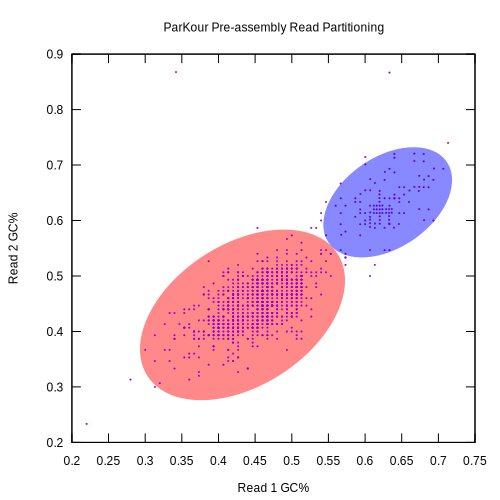
\includegraphics[width=\textwidth]{parKour.pdf}
    \caption{Plot of a random subsample of reads with their approximate cluster centroids overlaid as determined by parKour}
\end{figure}

The likely explanation for this is that even 150bp paired end reads are too short to consistently
statistically demonstrate the GC-AT bias of the originating organism. This means any partitioning
is likely to remove a significant number of reads necessary to complete transcripts due to local
variation in AT bias.  The high number of shorter contigs is indicative of the kind of assembly
fragmentation that would be expected in this situation.
    
\subsubsection{Assembly}

Referenced assembly using the divergent \textit{Chlorella NC64A},
\textit{Coccomyxa subellipsoidea} C-169, \textit{Tetrahymena thermophila},
\textit{Paramecium caudatum} genomes as references was largely fruitess.
Of all bulk and SCT reads only 0.3 and 0.4\% mapped to the 
algal references.  Similarly, only 0.6 and 0.9\% of reads mapped to the 
respective ciliate genomes.   This level of mapping is on the order
of random chance.  The high proportion of reads which mapped, mapped non-uniquely
suggesting mapping was occurring in low complexity reasons and is a statistical
artefact for the most part instead of biological significant.

Generally, spliced mapping like this can be improved by supplying 
gene junction annotation files for the genomes being mapped.
However, addition of GTF data only improved the percentage of reads mapping
by 0.05-0.3 percentage points.  With so few reads mapping, any attempt to 
class transcripts from this using cufflinks resulted in 10s of transcripts.

It is safe to conclude that despite other findings that even divergent 
(up to 15\%) genomes can generate transcriptomes of higher-quality
than \textit{de novo} \citep{Vijay2013}, the potential references
are too divergent in the case of the PbMr to be of any utility.


%We can calculate the probability of matches given
%random reads and a random 46.82Mb of host genome
%as a generalisation of the birthday 
%problem which asymptotically states
%\( p\equivalent 1 - exp(-n\frac{n-1}{2d})\)
%where \(d = 4^{100}\) i.e. the number of possible
%\(100bp\) 4-character reads and \(n =\) 
%

\textit{de novo} assembly 

\textbf{TOM: I am struggling how to best organise and present the mountain of assembly data and asssessment that has built up}

\begin{table}[h]
\begin{tabular}{|l|rrrrrrrl}
\hline
\multicolumn{1}{|c|}{Assembly} & \multicolumn{1}{c|}{Raw Reads (paired)} & \multicolumn{1}{c|}{\begin{tabular}[c]{@{}c@{}}Trimmed Reads \\ (assuming all paired)\end{tabular}} & \multicolumn{1}{c|}{Assembled Contigs} & \multicolumn{1}{c|}{Assembled "Genes"} & \multicolumn{1}{c|}{"Gene" N50} & \multicolumn{1}{c|}{"Gene" Mean Length} & \multicolumn{1}{c|}{"Gene" Total Assembled Bases} & \multicolumn{1}{c|}{GC\%} \\ \hline
Kodama Trinity                 & 232.3M                                  & 218.5M                                                                                              & 68,175                                 & 40,805                                 & 904                             & 1,832                                   & 36.9M                                             & \multicolumn{1}{c}{?}     \\ \cline{1-1}
SCT Q30                        & 126.9M                                  & 93.2M                                                                                               & 99,784                                 & 88,573                                 & 475                             & 451                                     & 40.0M                                             & 48.67                     \\ \cline{1-1}
SCT Q30 + Bulk                 & 179.4M                                  & 145.6M                                                                                              & 127,508                                & 103,506                                & 646                             & 564                                     & 58.2M                                             & 40.30                     \\ \cline{1-1}
SCT Q5                         & 126.9M                                  & 108.2M                                                                                              & 112,182                                & 99,441                                 & 465                             & 447                                     & 44.5M                                             & 49.42                     \\ \cline{1-1}
SCT Q5 + Bulk                  & 179.4M                                  & 160.6M                                                                                              & 139,226                                & 113,685                                & 615                             & 549                                     & 62.5M                                             & 41.28                     \\ \cline{1-1}
Bulk                           & 52.4M                                   & 52.4M                                                                                               & 43,261                                 & 30,706                                 & 1264                            & 861                                     & 26.5M                                             & 29.61                     \\ \cline{1-1}
\end{tabular}
\end{table}



%\subsubsection{Saturation}
%Trinity assemblies have been found to include more low-abundance k-mers than oases, many different isoforms
%but doesn't recover many more unique genes just more isoforms \citep{Lowe2014} 
%k-mer spectrum can be used to evaluate reocvoeery of low-abundance transcrtipts \citep{Pop2009}



To this end, the error corrected combined \textit{de novo} SCT light Q<5 trim and bulk assembly were selected for further analysis.
39,095 CDS sequences over 100aa in length were called from the 139,226 contigs using \textit{Tetrahymena} encoding.
%THIS IS NOT RIGHT

\subsection{Binning}



%Fortunately, to this end, the only other published 2nd generation sequencing analysis of \textit{P. bursaria} and a green algal,
%endosymbiont: Kodama \textit{et. al.} 2014 \citep{Kodama2014} partially addressed this issue.  This analysis investigated 
%the differential global metatranscriptome profile of \textit{P. bursaria} Yad1g strain with and without its \textit{Chlorella variabilis} 1N endosymbiont 
%\citep{Kodama2014}.   While, this is a different strain of both host and endosymbiont to the CCAP1660/12 strains (\textit{P. bursaria} and \textit{Micractinium reisseri}) 
%used in this thesis it offers a potential avenue to investigate these other components.
%An attempt was made to replicate this work using the CCAP1660/12 strains, unfortunately, elimination of the endosymbionts without death of the host
%didn't prove possible in these strains.  Despite using 
%
%(despite earlier publications to the contrary) by either maintaining the culture in the dark \citep{Siegel1960} (although some studies have thrown doubt on
%        how effective this method is at completely elimiating the photobiont \citep{Tanaka2002}) or treatment with various titrations of herbicides 
%            (e.g. paraquat \citep{Hosoya1995a}) or the protein synthesis inhibitor cyclohexamide \citep{weis1984effect}).\footnote{
%        There are naturally aposymbiotic strains of \textit{Paramecium bursaria} \citep{Tonooka2002a}}

From these, 39,095 contigs 18,111 were generated using ``Dendrogenous''.  Unfortunately, nearly half had too few hits in the 40 genomes used 
to generate phylogenies.  \footnote{However, in speed testing ``Dendrogenous'' did prove very efficient at rapidly generating phylogenies with its
fully parallelised mode capable of generating 100 phylogenies randomly selected transcripts against 41 genomes in an average 2:22.50 minutes.
The same pipeline run serially took an average of 23:41.39 minutes and the stage-wise parallel was very marginally faster at 
an average of 21:45.02 minutes.}



The initial identification and binning of recovered transcripts into host and endosymbiont categories was 
tested using this phylogenetic approach. The results of this analysis is plotted 
below. This demonstrates that the initial bin identifications were accurate for
endosymbiont (~92\%) and food ( ~94\%) derived transcripts. 
\textbf{This needs recalculated}
%Of the bins that were too large to
%be comprehensively phylogenetically tested (‘Host Bin’ and ‘Food Bin’) we screened a subset
%of 2000 transcripts using a phylogenomic approach. There were almost no detected endosym-
%biont sequences in 2000 randomly selected ‘Food Bin’ transcripts therefore the ‘Host Bin’ was
%the only cause for concern in containing misidentified endosymbiont transcripts. ~2\% of the
%2000 randomly sampled ‘Host Bin’ transcripts were found to be wrongly identified endosym-
%biont sequences, assuming this random sample is representative of the ‘Host Bin’ in general
%this suggests 500 endosymbiont transcripts are misidentified as host sequences.

\begin{figure}
    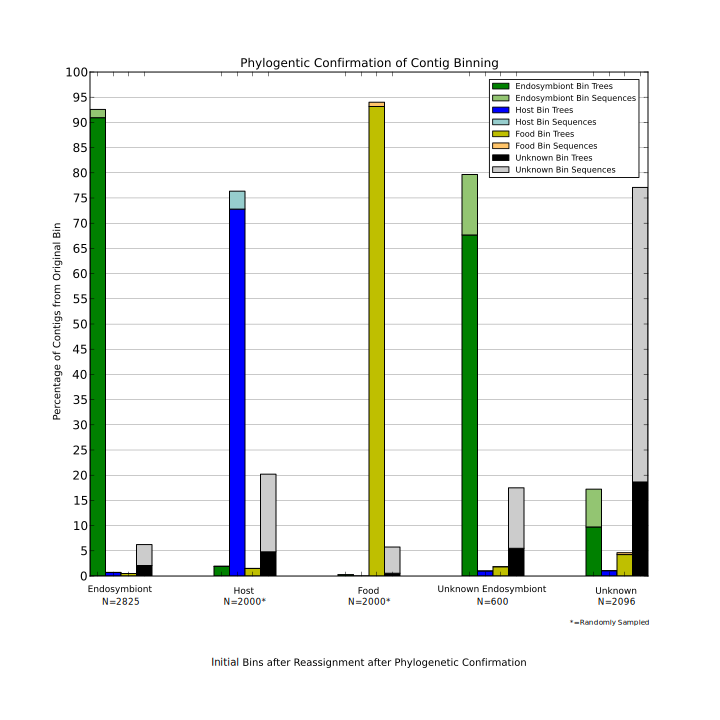
\includegraphics[width=\textwidth]{change_in_binning_after_phylogenetic_confirmation.pdf}
\end{figure}

For automated classification, the random forest test score showed a 93\% accuracy and automl approach ensemble test scored at 87.3\% accuracy.
Dishearteningly, this is not massively more accurate than the crude BLAST based binning approach.
     
\section{Conclusion}

In conclusion,
Library filtering is important with single cell possibly due to the increased inefficiency of poly-A selection
GC partitioning doesn't work - splits up contigs
Trimming and error correction makes little difference on unsaturated complex single cell 
Arboretum offers a useful way to accurately classify transcripts into likely origins 



